\section{Empirical Evaluation}

\label{sec:evaluation}

To evaluate our strategy, in this section we present the empirical study we conduct. Before explaining our study, we first introduce the terminology we use throughout this paper. In particular, we define in what follows four categories: abort, skip, fail, and pass.

\begin{itemize}

	\item \textbf{Abort:} students that aborted the course before the final exam;
	\item \textbf{Skip:} students that did not show up for the final exam, but were allowed to;
	\item \textbf{Fail:} students who failed the course;
	\item \textbf{Pass:} students who successfully passed the course.

	%\item \textbf{Abort:} the number of students aborting the course before the final exam;
	%\item \textbf{Skip:} the number of students not showing up for the final exam, but was allowed to;
	%\item \textbf{Fail:} the number of students who failed the course;
	%\item \textbf{Pass:} the number of students who passed the course.

\end{itemize}

Now, we present the objetives and hypotheses of our study, then the participants and material we use, and finally we detail the procedure we use during the evaluation.

\subsection{Objective and Hypotheses}

The objective of this study is to evaluate to what extent our strategy is capable of identifying potential failing students. This way, based on this objective, our hypotheses are the following:

\begin{itemize}

	\item \textbf{RH 1:} In the first 30 days, students with lower number of submissions and correct submissions tend to fail the course.

	\item \textbf{RH 2:} In the first 30 days, students with higher number of submissions and correct submissions tend to pass the course;

\end{itemize}

Although this paper focuses on identifying potential \textit{failing} students, we also study and report the opposite case according to our second hypothesis.

\subsection{Participants and Material}

The participants of our study consist of students of introductory programming courses at the Federal University of Alagoas, Brazil. We ministered these courses during 3.5 years and collected the results of each student by using Huxley. The professor informed all students that the use of Huxley was mandatory during the courses. Table~\ref{tab:participants} distribute the number of participants per semester.

\begin{table}[h]
\centering
\begin{tabular}{|c|c|}
\hline
\textbf{Course} & \textbf{Number of enrolled students}\\ \hline
2010.02 & 34\\ \hline
2011.01 & 38\\ \hline
2011.02 & 35\\ \hline
2012.01 & 34\\ \hline
2012.02 & 29\\ \hline
2013.01 & 28\\ \hline
2013.02 & 31\\ \hline
\end{tabular}
\caption{Participants per course.}
\label{tab:participants}
\end{table}

The material of this study consists of almost 300 programming exercises in Huxley. They were available to all students of all courses we use in this paper.

\subsection{Procedure}

\label{sec:procedure}

Figure~\ref{fig:procedure} illustrates how we proceed with our evaluation. The result of executing our strategy consists of three groups. Now, according to the groups, we have the potential failing students, the ones that have a small number of submissions and correct submissions (represented by circles). Notice we also have students that are potential candidates to successfully pass (represented by stars): after 30 days, they seem to be studying hard, due to the high number of submissions to Huxley.

\begin{figure}[htb]
\centering
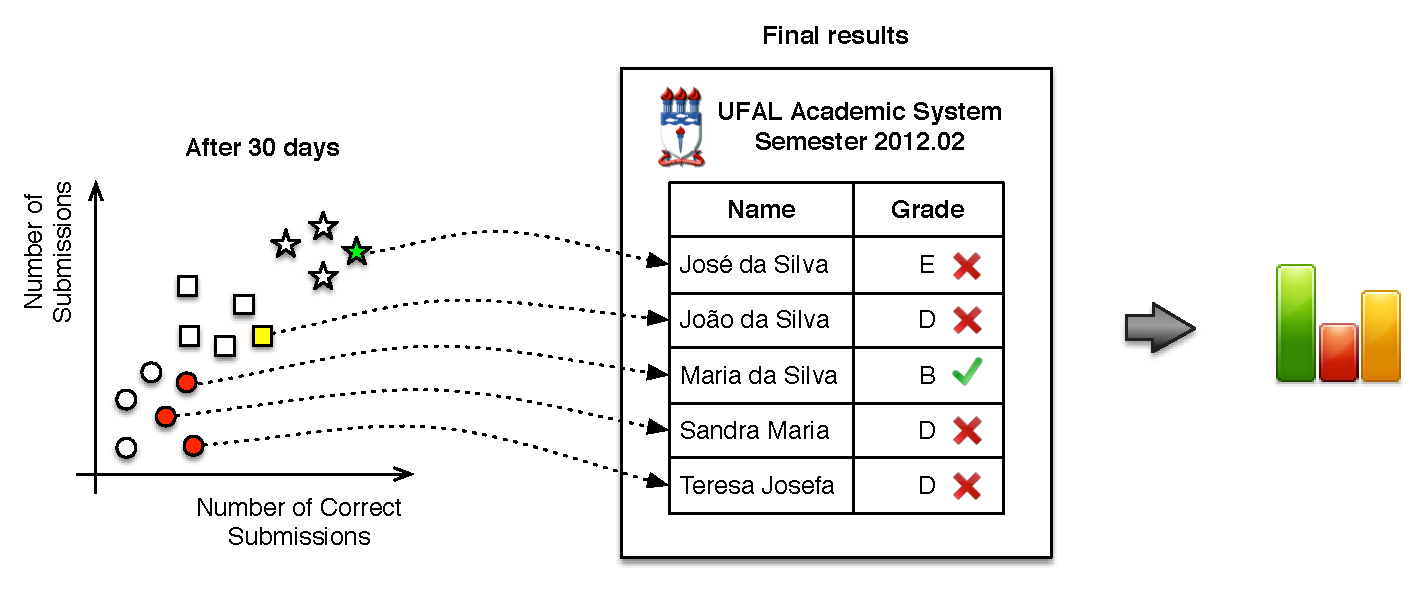
\includegraphics[width=1.0\textwidth,natwidth=610,natheight=642]{images/Procedure.pdf}
\caption{Checking the strategy results against the actual grades.}
\label{fig:procedure}
\end{figure}

After applying the clustering algorithm, we now need to check if the entire strategy correctly predicted the failing students. To do so, we use the academic system of the Federal University of Alagoas to look for grades and check whether the students passed or not. For example, for the detached circles, the strategy successfully identified that, after 30 days, both students would not pass and they indeed did not. Notice that the strategy may be analogously applied the other way around: when considering the detached star, the strategy identified that such a student would pass and she indeed passed.

\todo{Não estou conseguindo explicar bem a regra de associacao. Tem que melhorar muito mais isso!}

To better structure and analyze our results, we consider association rules~\cite{}, which take the form of $X \Rightarrow Y$, where $X$ and $Y$ are sets of items. In this paper, these items consist of students. Let $S$ be a set of students. The rules we consider are:

\begin{itemize}

	\item \textbf{Rule 1:} Strategy pointed $S$ as ``will Fail" $\Rightarrow$ $S$ indeed Failed

	\item \textbf{Rule 2:} Strategy pointed $S$ as ``will Pass" $\Rightarrow$ $S$ indeed Passed

\end{itemize}

To compute the strength or reliability of these rules, we use the confidence~\cite{}, which represents the probability of finding the right-hand side of the rule under the condition that these transactions contain the left-hand side as well. This way, the confidence is defined as follows:

$$
Confidence(X \Rightarrow Y) = \frac{Support(X \cup Y)}{Support(X)},
$$

where $Support$ is a function to \todots

Nevertheless, notice that our strategy is susceptible to yield false positives (the strategy pointed the student would pass, but she did not) and false negatives (the strategy pointed the student would not pass, but she did). We also consider these cases as well. %To compute these numbers, we consider Precision and Recall~\cite{}, as defined in what follows.

%\begin{align}
%x = y && 
%\end{align}

In summary, after confronting the strategy results with the academic system and summarizing all confidences, false negatives, and false positives, we apply statistical tests to check for significance. Here, we rely on the binomial statistical test based on the Bernoulli distribution~\cite{}.

\section{Results and Discussion}

In this section, we describe the results and test our hypotheses before discussing their implications (All data, materials, and R scripts are available at \url{http://www.ic.ufal.br/}). We now proceed separately, reporting the results where our strategy pointed out students who would fail the course and who would pass the course.

\subsection{Fail}

\begin{table}[h]
\centering
\begin{tabular}{|c|c|}
\hline
\textbf{Course} & \textbf{Confidence(Rule 1)}\\ \hline
2010.02 & 100\%\\ \hline
2011.01 & 84.62\% \\ \hline
2011.02 & 83.33\% \\ \hline
2012.01 & 75\% \\ \hline
2012.02 & 66.67\% \\ \hline
2013.01 & 58.33\% \\ \hline
2013.02 & 81.82\% \\ \hline
\end{tabular}
\caption{Confidences for the Rule 1 of Section~\ref{sec:procedure}.}
\label{tab:confidences}
\end{table}

\subsection{Pass}

\begin{table}[h]
\centering
\begin{tabular}{|c|c|}
\hline
\textbf{Course} & \textbf{Confidence(Rule 2)}\\ \hline
2010.02 & 33.33\% \\ \hline
2011.01 & 100\%  \\ \hline
2011.02 & 88.89\% \\ \hline
2012.01 & 50\%  \\ \hline
2012.02 & 66.67 \\ \hline
2013.01 & 100\% \\ \hline
2013.02 & 100\% \\ \hline
\end{tabular}
\caption{Confidences for the Rule 2 of Section~\ref{sec:procedure}.}
\label{tab:confidences}
\end{table}

\subsection{Discussion}

\begin{itemize}

	\item Olhar se, para os alunos onde o algoritmo errou, eles foram pra prova final.
	\item Olhar se, para os alunos onde o algoritmo acertou, quantos deles falharam.

\end{itemize}

\subsection{Threats to validity} 